\section{Messmodi}
Sowohl der Fußschalter als auch der USB-Dongle sollen in mehreren verschiedenen Operationsmodi laufen können. Dieser wird in einer zusätzlichen globalen Konfigurationsdatei spezifiziert. Zum Zeitpunkt der Implementierung der USB-App war die App die oberste Abstraktionsschicht aller USB-Funktionalität. Das ist mit Einführung der Fußschalter Funktionalitäten nicht mehr der Fall. Daher bedarf es einer neuen Abstraktionsschicht, die über der Dongle- und Fußschalterapp steht und die Funktionalitäten beider dirigiert. Dadurch können die Operationsmodi programmatisch getrennt werden, sodass bestimmte Schritte der Initialisierung, wie das Einlesen der Konfigurationsdatei der zu verbindenden Geräte, in einem Modus wie \ac{HID} einzelnes Zeichen nicht ausgeführt werden. Zum Ende dieser Arbeit sind folgende Modi konfigurierbar:
\begin{itemize}
	\item 0: USB-\ac{HID}-singleKey
	\item 1: USB-\ac{HID}
	\item 2: CDC (COM-Port)
	\item 3: \ac{BLE}-\ac{HID}
	\item 4: \ac{BLE}-\ac{HID}-singleKey
\end{itemize}

\begin{figure}[H] 
	\centering
	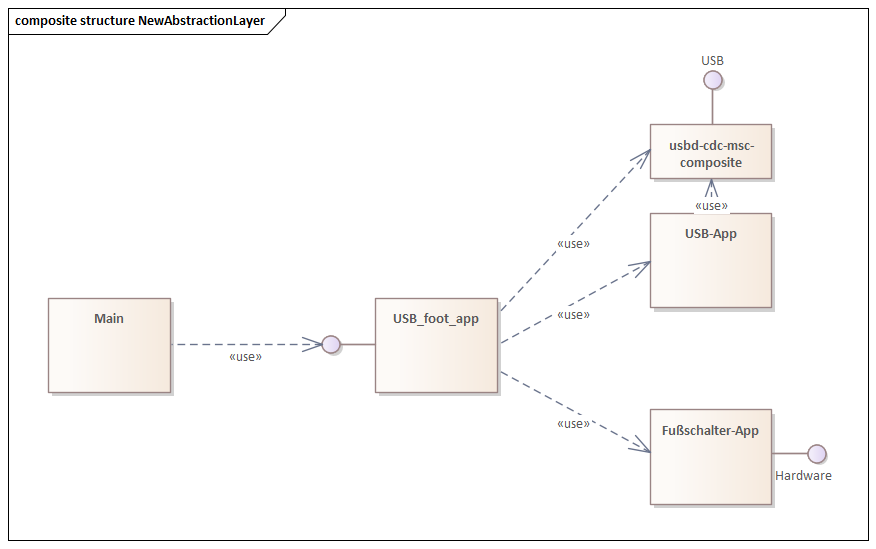
\includegraphics[width=\textwidth]{figures/NewAbstractionLayer.png}
	\caption{Neue Abstraktionsschicht}
\end{figure}

\subsection{USB-HID}
Ein Feature, das sowohl für den Dongle als auch für den Fußschalter implementiert werden soll, ist das Human Interface Device (HID) über USB. In diesem Modus gibt die Anwendung die Messergebnisse nicht mehr über den virtuellen COM-Port aus, sondern ist über USB als Tastatur mit dem Computer verbunden. Über sie werden die Zeichen der Messung als Tastendrücke, gefolgt von einem konfigurierbaren Terminierungszeichen, ausgegeben. Dadurch können Messungen einfach in Excel oder einem Texteditor aufgefangen werde.\\
Für die Implementierung werden die Funktionen des NRF-Library Files app\_usb\_hid\_kbd.h verwendet. Es abstrahiert die Low-Level USB-Aufrufe und stellt Funktionen zur Verfügung, die bei Aufruf eine Taste drücken oder loslassen. Es fehlt jedoch eine Funktion die ganze Strings serialisiert, weshalb diese implementiert werden muss. Die Scancodes, die Nummern der Tasturtasten, sowie der Modifier, eine Taste die Tastendrücke modifiziert, wie die Shift-Taste, werden dabei von einer Funktion erhalten, die im nrf\_Base Projekt enthalten ist. Sie wurde für die \ac{HID} Implementierung über \ac{BLE} geschrieben und gibt den Scancode und zugehörigen Modifier für einen ASCII Character zurück.\\
Zwischen den Tastendrücken muss eine gewisse Zeit gewartet werden, da der Computer Tastendrücke zwischen denen zu wenig Zeit verstreicht nicht registriert. Dieser Delay wurde auf 1 Millisekunden festgelegt, da bei einem längeren Delay die Anzahl an fehlerhaften Tastendrücken zunahm. Diese Art darauf zu warten, dass die Tastendrücke vom Computer registriert wurde, stellte sich jedoch als sehr fehleranfällig heraus. Nicht nur wurde dopplete Zeichen nicht korrekt erkannt, sondern nach ungefähr 10 Ausgaben schien der USB-Bus überlastet zu sein. Daher musste die Implementierung geändert werden. Statt die Tastendrücken ohne Rücksicht auf die zugehörigen Events dem USB zu übergeben, muss nach jedem Zeichen auf ein Event der USB-\ac{HID} Library gewartet werden, das die erfolgreiche Übertragung signalisiert. Dazu muss der zu serialisierende String in einem Buffer hinterlegt und bei Empfangen des Events das nächste Zeichen übertragen werden.\\
Eine Abwandlung dieses Modus, ist der Modus USB-\ac{HID}-singleKey. In diesem Modus gibt der Fußschalter bei Betätigung des Tasters nur ein einzelnes kofigurierbares Zeichen aus, beziehungsweise bei einem Doppelklick ein Zweites, wie in Abschnitt 5.2 beschrieben ist.

\subsection{BLE-HID}
Ein weiterer Modus, in dem der Fußschalter arbeiten soll, ist \ac{HID} über \ac{BLE}. Dabei simuliert der Fußschalter oder Dongle eine über \ac{BLE} verbindbare Tastatur und serialisiert nach dem Verbinden wie bei \ac{HID} über USB die Messergebnisse als Tastendrücken. Dazu muss das Gerät nun zusätzlich zur Central Rolle in der Peripheral Rolle agieren. Dazu muss einerseits das Advertising korrekt konfiguriert werden und in den bestehenden Code des Peripheren Verbindungsaufbaus, die Fußschalter Applikation eingebunden werden. Für das eigentliche Schreiben des Messergebnisses über \ac{BLE}, gibt es bereits eine bestehenden Funktionen des nrf\_Base Projekts die einen String vollständig serialisiert und diese muss nur in der Fußschalter Applikation aufgerufen werden.\\
Dabei erfordert dieser Modus es nun, dass die Bonding Informationen der Verbindung von Fußschalter zu Computer gelöscht werden kann. Werden sie nicht gelöscht, jedoch auf dem Computer, können sich die beiden Geräte nicht mehr miteinander verbinden. Das muss zum Beispiel geschehen, wenn der Fußschalter mit einem anderen Computer verbunden werden soll, sich der erste Computer jedoch noch in Reichweite befindet. Trotzdem sollen nicht bei jedem Reset des Fußschalter, also bei einer Änderung der Konfigurationsdatei, die Bonding Informationen gelöscht werden, da sonst bei jedem Verbinden, der Fußschalter im Computer erst entkoppelt und dann wieder neugekoppelt werden muss. Es kann also nicht direkt gesagt werden wann die Bonding Informationen gelöscht werden sollen und wann nicht, stattdessen wäre der Idealfall, dass der User selbst die Informationen löschen kann. Das ist jedoch aufgrund der begrenzten Interaktionsmöglichkeiten des Users mit dem Fußschalter nur schwierig umsetzbar. Ein Kompromiss ist, dass die Bonding Informationen gelöscht werden, wenn der Modus \ac{BLE}-\ac{HID} verlassen wird. Der Anwender kann dann auch um die Bonding Informationen zu löschen aus dem Modus 3 herauswechseln und dann wieder hineinwechseln. Dabei ist das Problem, dass bei einem Reset nicht direkt ersichtlich ist, in welchen Modus gewechselt wird, da die Konfigurationsdatei erst beim Neutstart neugelesen wird. Daher wird direkt vor dem Reset die Konfigurationsdatei gelesen und falls aus dem Modus 3 oder 4 in einen anderen Modus gewechselt wird, die Bonding Informationen gelöscht. Ein alternativer Lösungansatz der ohne das ressourcenfordernde Einlesen der Datei auskommt, ist die Bonding Informationen immer zu löschen, wenn sich der Fußschalter beim Reset in einem anderen Modus als 3 oder 4 befindet. Jedoch war dann der ``Peer Manager'' nicht initialisiert, der zum Löschen der Bonding Informationen zwingend benötigt wird, weshalb doch der erste Lösungansatz umgesetzt wurde. Der Peer Manager ist dabei eine Library von NRF die sich um Verschlüssung, Pairing und Bonding kümmert (\cite[]{NRF_PeerManager}).\\
Erste Tests zeigen, dass die Geschwindigkeit der Übertragung, einerseits die Dauer bis zum ersten Tastendruck und anderseits die Zeit zwischen den einzelnen Tastendrücken, zu hoch ist. Die Untersuchung wo genau zuviel Zeit verwendet wird, fand mithilfe eines Oszilloskop und dem togglen eines freien Pins, der zu diesen Debugzweck belegt wurde, statt. Es konnte dadurch bereits ein Bug im nrf\_Base Projekt gefunden werden. Dabei wird in der Funktion, zwischen den einzelnen Zeichen eine Pause gemacht, um ähnlich im Modus USB-\ac{HID} dem Betriebssystem Zeit zu geben die Tastendrücke zu verarbeiten. Dieser Delay ist abhängig von Connection Interval, welches wenn nur die Verbindung zum Computer besteht, korrekt gesetzt ist. Jedoch stellte sich heraus, dass diese globale Variable von allen Verbindungen stets überschrieben wird. Dabei ist diese Variable auch unabhängig von der \ac{HID} Funktionalität nur für die peripheren Verbindungen von Bedeutung und dieses Verhalten ein Fehler. Es wurde daher an der Stelle, an der diese Variable durch einen ``Connection Update Request'' überschrieben wird, die Unterscheidung eingeführt, ob es sich bei der Verbindung um eine periphere Verbindung handelt.\\
Auch von diesem Modus, gibt es die Abwandlung \ac{BLE}-\ac{HID}-singleKey, die wie im Modus USB-\ac{HID}-singleKey, ein einzelnes Zeichen bei Betätigung des Tasters ausgibt.

\subsection{BLE-HCT-Windows-App}
Der letzte Modus, in dem der Fußschalter agieren soll, ist als ein an die \ac{HCT}-Windows-App angebundenes Gerät. Dabei soll das Signal der Betätigung des Tasters als eine \ac{HCT}-Nachricht an die Windows-App gesendet werden, welchen dann ein Messergebnis bei den mit ihr verbundenen Messgeräten triggert. Dazu muss ein \ac{HCT}-Model für den Fußschalter geschaffen werden. Das Model stellt folgende Werte bereit:
\begin{itemize}
	\item Device Class
	\item Protocol type, version 
	\item Version of Hardware, Software, \ac{BLE}
	\item Battery level, status
	\item Reset 
\end{itemize}

Werte des Config.ini Konfigurationsfiles:
\begin{itemize}
	\item Operating Mode 
	\item CDC protocol 
	\item HID Keyboard Language ID 
	\item HID data set seperator 
	\item HID number seperator
	\item HID single key 
\end{itemize}

Für die Übertragung des eigentlichen Signals, dass der Fußschalter betätigt wurde, muss eine \ac{HCT}-Charakteristik angelegt werden, auf welche die \ac{HCT}-Windows-App sich subscriben kann. Über diese Charakteristik wird sie dann über die Betätigung des Tasters notifiziert. Im Advertising muss sich der Fußschalter dann nicht als Tastatur, sondern als \ac{HCT}-Fußschalter erkenntlich zeigen.\\
Es wurde jedoch beschlossen, diesen Modus erst in einer späteren Version des Fußschalters zu implementieren, wie im Abschnitt 8.2 genauer erklärt wird.